\documentclass{article}

\usepackage[letterpaper, top=2cm, bottom=1cm, inner=1.8cm,
outer=1.8cm, foot=1cm]{geometry}

\setcounter{tocdepth}{1}

\usepackage{amsmath, amssymb}
\usepackage{comment}
\usepackage{graphicx}
%\usepackage[T1]{fontenc}
%\usepackage{ae, aecompl}
\usepackage[numbers]{natbib}

%%%%%%%%%%%%%%%%%%%%%%%%%%%%%%%%%%%%%%%%%%%%%%%%%%%%%%%%%%%%%%%%%%%%%%%%
%% math

%
% General
%

\DeclareMathOperator{\argmin}{arg\,min}
\DeclareMathOperator{\argmax}{arg\,max}

%
% Sets
%

\newcommand{\card} [1]{{\lvert #1 \rvert}}
\newcommand{\range}[1]{{\left\{ 1, \dots, #1 \right\}}}

%
% Linear algebra
%

\newcommand{\mat}  [1]{{\bf #1}}
\newcommand{\norm} [1]{{\lVert #1 \rVert}}
\newcommand{\vect} [1]{{\mbox{\boldmath $#1$}}}

%
% Probability. The CTAN `proba` package doesn't seem to be that good.
% TODO ensuremath does not seem to be a good idea.
%

\newcommand{\E}    [2]{{\textrm{E} \left[ #1 \mid #2 \right]}}
\newcommand{\LL}   [2]{{\ensuremath{ L \left( #1 \,\middle|\, #2 \right) }}}
\newcommand{\LLL}  [2]{{\ensuremath{ l \left( #1 \,\middle|\, #2 \right) }}}
\newcommand{\N}    [1]{{\ensuremath{ \# \left( \textrm{ #1 } \right) }}}
\newcommand{\PO}   [1]{{\Pr \left( #1 \right)}}
\newcommand{\PP}   [2]{{\PO{ #1 \,\middle|\, #2 }}}

%%%%%%%%%%%%%%%%%%%%%%%%%%%%%%%%%%%%%%%%%%%%%%%%%%%%%%%%%%%%%%%%%%%%%%%%
%% Theoretical computer science

%
% Computational complexity
%

\DeclareMathOperator{\bigO}{O}
\providecommand{\OO}[1]{\bigO\bigl(#1\bigr)}

%%%%%%%%%%%%%%%%%%%%%%%%%%%%%%%%%%%%%%%%%%%%%%%%%%%%%%%%%%%%%%%%%%%%%%%%
%% General text

% \emph toggles italics; \textit sets italics; \em is deprecated
\newcommand{\term} [1]{{\emph{#1\/}}} 

% We don't need to do append a ~ or \ because TeX already handles .,
% correctly. TODO figure out if italics are correct here
\newcommand{\foreign}[1]{{\textit{#1}}}
\newcommand{\ea}      {{\foreign{et~al.}}}
\newcommand{\eg}      {{\foreign{e.g.}}}
\newcommand{\ie}      {{\foreign{i.e.}}}
\newcommand{\TODO} [1]{{\textbf{TODO}: \textit{#1}}}

%%%%%%%%%%%%%%%%%%%%%%%%%%%%%%%%%%%%%%%%%%%%%%%%%%%%%%%%%%%%%%%%%%%%%%%%
%% Remarks. Collected from the pervasive but untraceable `remarks.tex`.

\newif\ifremark
\long\def\remark#1{
\ifremark%
    \begingroup%
    \dimen0=\columnwidth
    \advance\dimen0 by -0.25in%
    \setbox0=\hbox{\parbox[b]{\dimen0}{\protect\em\textcolor{red}{#1}}}
    \dimen1=\ht0\advance\dimen1 by 2pt%
    \dimen2=\dp0\advance\dimen2 by 2pt%
    \vskip 0.25pt%
    \hbox to \columnwidth{%
        \vrule height\dimen1 width 3pt depth\dimen2%
        \hss\copy0\hss%
        \vrule height\dimen1 width 3pt depth\dimen2%
    }%
    \endgroup%
\fi}

\newcommand{\remarkname}[2] {
    \remark{{\bf #1}:#2}
}


\def\LaTeXe{c}

\title{Collaborative Filtering for the Netflix Prize}
\author{Masahiro Ono and Yang Zhang}

\begin{document}

\maketitle

\tableofcontents

\section{Introduction}

\subsection{Project Overview}

We implemented and evaluated two approaches to collaborative
filtering: mixture model MLE and low-rank approximation. We analyze
these approaches and evaluate them on a subset of the Netflix Prize
data set. This report includes the theoretical basis of each approach
and the empirical results of our experimental evaluation as well as
complexity analysis and discussion of their feasibility for
larger-scale problems.

\TODO{two methods are kind of opposite}

\subsection{Dataset}

The Netflix data set is large: it contains 480,189 users, 17,770
movies, and 100,480,507 ratings. MATLAB's in-memory data management is
not amenable to data sets of such scale, and working with such a large
data set incurs implementation challenges that are beyond the scope of
our class project. Hence, we use a much smaller subset of the full
Netflix Prize data set consisting of 51 movies and 892 users, chosen so
that the resulting rating matrix is fully packed. We then divide the
rating matrix into training and test data. Since we have the fully
packed rating matrix, we can arbitrary specify the \term{sparsity
  ratio}\footnote{\textit{The sparsity ratio is the ratio of missing
    ratings to the size of the matrix. The original Netflix Prize data
    has a sparsity ratio of 99\%.}} of the training data to evaluate
the dependency of the performance on the sparsity ratio.

In this report, we denote by $\mat{R}$ the rating matrix whose rows
correspond to users and columns correspond to movies, such that entry
$r_{i,j} \in \range{5}$ is the rating given by user $i$ to movie
$j$. We also denote by $n_U$ and $n_M$ the number of users and movies.

\subsection{Performance Measure}
The performance of each algorithm is measured by root-mean-square
error,
\begin{equation}
  \textrm{RMSE} = \left[
    \sum_{(i,j) \in I_T} ({\hat r}_{i,j} - r_{i,j})^2
  \right]^\frac{1}{2}
\end{equation}
where $I_T$ is the set of indexes of the ratings included in the test
data and ${\hat r}_{i,j}$ is the estimated rating of $i$th user for
$j$th movie.

\section{Mixture Model}

We use a mixture model to cluster together ratings based on user types
and movie types. There are various other mixture models for
collaborative filtering; this model is the one presented in 6.867
lecture 15 and is known as the \term{flexible mixture
  model}~\cite{si03flexible}. A survey of various alternative models
can be found in~\cite{cmu-study}.

For this part of our project, we rigorously derived the E-M algorithm,
implement the algorithm in MATLAB, and analyzed its results. In the
following sections, we describe and justify the model, then derive the
E-M algorithm and analyze its complexity. Next, we describe our
implementation, and finally we evaluate its RMSE
performance. Throughout these sections, we will identify key
variables, but also provide complete definitions in the appendix for
the reader's reference.

\subsection{Overview}

We say that \term{each user} has a distribution over user types (\eg,
mostly romantic, a bit of an intellectual), and each movie has a
distribution over movie types (mostly horror, some action). Each pair
of user type and movie type has a distribution over ratings (\eg,
romantics tend to give horrors low ratings). The likelihood of
our model given the parameters is then
\begin{align}
  \LL{D}{\theta}
  =& \PP{ R_{1,1} = r_{1,1}, \dots, R_{n_U,n_M} = r_{n_U,n_M} }{
    \theta } \\
  =& \prod_{i,j} \sum_{u,m} \left[
    \PP{ R_{i,j} = r_{i,j} }{ U_{i,j} = u, M_{i,j} = m,
      \theta^R_{u,m} } \cdot 
    \PP{ U_{i,j} = u }{ \theta^U_i } \cdot
    \PP{ M_{i,j} = m }{ \theta^M_j }
  \right] \\
  =& \prod_{i,j} \sum_{u,m}
  \theta^R_{u,m}(r) \cdot \theta^U_i(u) \cdot \theta^M_j(m)
\end{align}
We see that there are three sets of parameters, and our approach is to
use an E-M algorithm to perform maximum likelihood estimation of these
parameters. A graphical model representation of our mixture model is
in figure~\ref{fig:graphical}.

Each cell has its own user type and movie type. What does all this
mean?  Intuitively, we can think of each cell as the result of an
\term{act} of rating. Hence, every time a user rates a movie, we are
randomly sampling from among the user's multiple personalities (\eg,
the romantic in the user was rating this movie). We are also sampling
from among the movie's multiple aspects (the user saw this movie as a
horror movie). We will loosely use the term ``rating'' to mean either
the act of the rating or the rating value itself; hopefully the
meaning remains clear from the context.

It is natural to use multinomial distributions for generating the user
types for a user, and the movie types for a movie. We are also using
multinomial distributions to generate ratings given a user type and
movie type; this we do for simplicity. We discuss this further in
section \ref{sec:comparison}.

\begin{figure}[ht]
  \begin{center}
    % Graphic for TeX using PGF
% Title: /home/yang/work/netflix/doc/report/mixture2.dia
% Creator: Dia v0.96.1
% CreationDate: Tue Dec  4 17:14:11 2007
% For: yang
% \usepackage{tikz}
% The following commands are not supported in PSTricks at present
% We define them conditionally, so when they are implemented,
% this pgf file will use them.
\ifx\du\undefined
  \newlength{\du}
\fi
\setlength{\du}{15\unitlength}
\begin{tikzpicture}
\pgftransformxscale{1.000000}
\pgftransformyscale{-1.000000}
\definecolor{dialinecolor}{rgb}{0.000000, 0.000000, 0.000000}
\pgfsetstrokecolor{dialinecolor}
\definecolor{dialinecolor}{rgb}{1.000000, 1.000000, 1.000000}
\pgfsetfillcolor{dialinecolor}
\pgfsetlinewidth{0.010000\du}
\pgfsetdash{}{0pt}
\pgfsetdash{}{0pt}
\pgfsetmiterjoin
\pgfsetbuttcap
\definecolor{dialinecolor}{rgb}{0.000000, 0.000000, 0.000000}
\pgfsetstrokecolor{dialinecolor}
\draw (22.500000\du,8.000000\du)--(31.000000\du,16.500000\du)--(25.400000\du,22.100000\du)--(16.900000\du,13.600000\du)--cycle;
\pgfsetlinewidth{0.010000\du}
\pgfsetdash{}{0pt}
\pgfsetdash{}{0pt}
\pgfsetmiterjoin
\pgfsetbuttcap
\definecolor{dialinecolor}{rgb}{0.000000, 0.000000, 0.000000}
\pgfsetstrokecolor{dialinecolor}
\draw (28.500000\du,8.000000\du)--(34.100000\du,13.700000\du)--(25.600000\du,22.100000\du)--(20.000000\du,16.500000\du)--cycle;
\definecolor{dialinecolor}{rgb}{1.000000, 1.000000, 1.000000}
\pgfsetfillcolor{dialinecolor}
\pgfpathellipse{\pgfpoint{19.500000\du}{13.500000\du}}{\pgfpoint{0.500000\du}{0\du}}{\pgfpoint{0\du}{0.500000\du}}
\pgfusepath{fill}
\pgfsetlinewidth{0.010000\du}
\pgfsetdash{}{0pt}
\pgfsetdash{}{0pt}
\definecolor{dialinecolor}{rgb}{0.000000, 0.000000, 0.000000}
\pgfsetstrokecolor{dialinecolor}
\pgfpathellipse{\pgfpoint{19.500000\du}{13.500000\du}}{\pgfpoint{0.500000\du}{0\du}}{\pgfpoint{0\du}{0.500000\du}}
\pgfusepath{stroke}
\definecolor{dialinecolor}{rgb}{1.000000, 1.000000, 1.000000}
\pgfsetfillcolor{dialinecolor}
\pgfpathellipse{\pgfpoint{22.500000\du}{16.500000\du}}{\pgfpoint{0.500000\du}{0\du}}{\pgfpoint{0\du}{0.500000\du}}
\pgfusepath{fill}
\pgfsetlinewidth{0.010000\du}
\pgfsetdash{}{0pt}
\pgfsetdash{}{0pt}
\definecolor{dialinecolor}{rgb}{0.000000, 0.000000, 0.000000}
\pgfsetstrokecolor{dialinecolor}
\pgfpathellipse{\pgfpoint{22.500000\du}{16.500000\du}}{\pgfpoint{0.500000\du}{0\du}}{\pgfpoint{0\du}{0.500000\du}}
\pgfusepath{stroke}
\definecolor{dialinecolor}{rgb}{1.000000, 1.000000, 1.000000}
\pgfsetfillcolor{dialinecolor}
\pgfpathellipse{\pgfpoint{25.500000\du}{19.500000\du}}{\pgfpoint{0.500000\du}{0\du}}{\pgfpoint{0\du}{0.500000\du}}
\pgfusepath{fill}
\pgfsetlinewidth{0.010000\du}
\pgfsetdash{}{0pt}
\pgfsetdash{}{0pt}
\definecolor{dialinecolor}{rgb}{0.000000, 0.000000, 0.000000}
\pgfsetstrokecolor{dialinecolor}
\pgfpathellipse{\pgfpoint{25.500000\du}{19.500000\du}}{\pgfpoint{0.500000\du}{0\du}}{\pgfpoint{0\du}{0.500000\du}}
\pgfusepath{stroke}
\definecolor{dialinecolor}{rgb}{1.000000, 1.000000, 1.000000}
\pgfsetfillcolor{dialinecolor}
\pgfpathellipse{\pgfpoint{28.500000\du}{16.500000\du}}{\pgfpoint{0.500000\du}{0\du}}{\pgfpoint{0\du}{0.500000\du}}
\pgfusepath{fill}
\pgfsetlinewidth{0.010000\du}
\pgfsetdash{}{0pt}
\pgfsetdash{}{0pt}
\definecolor{dialinecolor}{rgb}{0.000000, 0.000000, 0.000000}
\pgfsetstrokecolor{dialinecolor}
\pgfpathellipse{\pgfpoint{28.500000\du}{16.500000\du}}{\pgfpoint{0.500000\du}{0\du}}{\pgfpoint{0\du}{0.500000\du}}
\pgfusepath{stroke}
\definecolor{dialinecolor}{rgb}{1.000000, 1.000000, 1.000000}
\pgfsetfillcolor{dialinecolor}
\pgfpathellipse{\pgfpoint{31.500000\du}{13.500000\du}}{\pgfpoint{0.500000\du}{0\du}}{\pgfpoint{0\du}{0.500000\du}}
\pgfusepath{fill}
\pgfsetlinewidth{0.010000\du}
\pgfsetdash{}{0pt}
\pgfsetdash{}{0pt}
\definecolor{dialinecolor}{rgb}{0.000000, 0.000000, 0.000000}
\pgfsetstrokecolor{dialinecolor}
\pgfpathellipse{\pgfpoint{31.500000\du}{13.500000\du}}{\pgfpoint{0.500000\du}{0\du}}{\pgfpoint{0\du}{0.500000\du}}
\pgfusepath{stroke}
\definecolor{dialinecolor}{rgb}{1.000000, 1.000000, 1.000000}
\pgfsetfillcolor{dialinecolor}
\pgfpathellipse{\pgfpoint{20.000000\du}{19.500000\du}}{\pgfpoint{0.500000\du}{0\du}}{\pgfpoint{0\du}{0.500000\du}}
\pgfusepath{fill}
\pgfsetlinewidth{0.010000\du}
\pgfsetdash{}{0pt}
\pgfsetdash{}{0pt}
\definecolor{dialinecolor}{rgb}{0.000000, 0.000000, 0.000000}
\pgfsetstrokecolor{dialinecolor}
\pgfpathellipse{\pgfpoint{20.000000\du}{19.500000\du}}{\pgfpoint{0.500000\du}{0\du}}{\pgfpoint{0\du}{0.500000\du}}
\pgfusepath{stroke}
\pgfsetlinewidth{0.010000\du}
\pgfsetdash{}{0pt}
\pgfsetdash{}{0pt}
\pgfsetbuttcap
{
\definecolor{dialinecolor}{rgb}{0.000000, 0.000000, 0.000000}
\pgfsetfillcolor{dialinecolor}
% was here!!!
\pgfsetarrowsend{stealth}
\definecolor{dialinecolor}{rgb}{0.000000, 0.000000, 0.000000}
\pgfsetstrokecolor{dialinecolor}
\draw (19.853553\du,13.853553\du)--(22.146447\du,16.146447\du);
}
\pgfsetlinewidth{0.010000\du}
\pgfsetdash{}{0pt}
\pgfsetdash{}{0pt}
\pgfsetbuttcap
{
\definecolor{dialinecolor}{rgb}{0.000000, 0.000000, 0.000000}
\pgfsetfillcolor{dialinecolor}
% was here!!!
\pgfsetarrowsend{stealth}
\definecolor{dialinecolor}{rgb}{0.000000, 0.000000, 0.000000}
\pgfsetstrokecolor{dialinecolor}
\draw (22.853553\du,16.853553\du)--(25.146447\du,19.146447\du);
}
\pgfsetlinewidth{0.010000\du}
\pgfsetdash{}{0pt}
\pgfsetdash{}{0pt}
\pgfsetbuttcap
{
\definecolor{dialinecolor}{rgb}{0.000000, 0.000000, 0.000000}
\pgfsetfillcolor{dialinecolor}
% was here!!!
\pgfsetarrowsend{stealth}
\definecolor{dialinecolor}{rgb}{0.000000, 0.000000, 0.000000}
\pgfsetstrokecolor{dialinecolor}
\draw (28.146447\du,16.853553\du)--(25.853553\du,19.146447\du);
}
\pgfsetlinewidth{0.010000\du}
\pgfsetdash{}{0pt}
\pgfsetdash{}{0pt}
\pgfsetbuttcap
{
\definecolor{dialinecolor}{rgb}{0.000000, 0.000000, 0.000000}
\pgfsetfillcolor{dialinecolor}
% was here!!!
\pgfsetarrowsend{stealth}
\definecolor{dialinecolor}{rgb}{0.000000, 0.000000, 0.000000}
\pgfsetstrokecolor{dialinecolor}
\draw (31.146447\du,13.853553\du)--(28.856973\du,16.143027\du);
}
% setfont left to latex
\definecolor{dialinecolor}{rgb}{0.000000, 0.000000, 0.000000}
\pgfsetstrokecolor{dialinecolor}
\node[anchor=west] at (23.000000\du,16.500000\du){$U$};
% setfont left to latex
\definecolor{dialinecolor}{rgb}{0.000000, 0.000000, 0.000000}
\pgfsetstrokecolor{dialinecolor}
\node[anchor=west] at (22.500000\du,16.500000\du){};
% setfont left to latex
\definecolor{dialinecolor}{rgb}{0.000000, 0.000000, 0.000000}
\pgfsetstrokecolor{dialinecolor}
\node[anchor=west] at (29.000000\du,16.500000\du){$M$};
% setfont left to latex
\definecolor{dialinecolor}{rgb}{0.000000, 0.000000, 0.000000}
\pgfsetstrokecolor{dialinecolor}
\node[anchor=west] at (26.000000\du,19.500000\du){$R$};
% setfont left to latex
\definecolor{dialinecolor}{rgb}{0.000000, 0.000000, 0.000000}
\pgfsetstrokecolor{dialinecolor}
\node[anchor=west] at (20.000000\du,13.500000\du){$\theta^U$};
% setfont left to latex
\definecolor{dialinecolor}{rgb}{0.000000, 0.000000, 0.000000}
\pgfsetstrokecolor{dialinecolor}
\node[anchor=west] at (32.000000\du,13.500000\du){$\theta^M$};
% setfont left to latex
\definecolor{dialinecolor}{rgb}{0.000000, 0.000000, 0.000000}
\pgfsetstrokecolor{dialinecolor}
\node[anchor=west] at (20.000000\du,20.500000\du){$\theta^R$};
% setfont left to latex
\definecolor{dialinecolor}{rgb}{0.000000, 0.000000, 0.000000}
\pgfsetstrokecolor{dialinecolor}
\node[anchor=west] at (20.000000\du,11.500000\du){$i \in \range{n_U}$};
% setfont left to latex
\definecolor{dialinecolor}{rgb}{0.000000, 0.000000, 0.000000}
\pgfsetstrokecolor{dialinecolor}
\node[anchor=west] at (27.000000\du,11.500000\du){$j \in \range{n_M}$};
\pgfsetlinewidth{0.010000\du}
\pgfsetdash{}{0pt}
\pgfsetdash{}{0pt}
\pgfsetbuttcap
{
\definecolor{dialinecolor}{rgb}{0.000000, 0.000000, 0.000000}
\pgfsetfillcolor{dialinecolor}
% was here!!!
\pgfsetarrowsend{stealth}
\definecolor{dialinecolor}{rgb}{0.000000, 0.000000, 0.000000}
\pgfsetstrokecolor{dialinecolor}
\draw (20.500000\du,19.500000\du)--(25.000000\du,19.500000\du);
}
\end{tikzpicture}

  \end{center}
  \caption{A graphical model representation of our mixture model.}
  \label{fig:graphical}
\end{figure}

Note that this model works for collaborative filtering for a static
set of users and movies (filling in holes). New users/movies
(augmenting our matrix with rows/columns that contain no data) would
indeed be difficult to provide recommendations for regardless of
model. However, even if these new rows/columns had data available, our
approach requires re-training the model, because each user and each
movie has its own distribution over user types and movie types.

\subsection{E-M Algorithm}

\subsubsection{M-step with complete data}

To derive the E-M algorithm, it is helpful to start by assuming that
we have ``complete data''---that is, for each of the (observed)
ratings $i,j$, we know precisely which user type $u$ and movie type
$m$ the rating belongs to. With this information, we can directly and
analytically find the parameters that maximize the likelihood of the
data. We can equivalently optimize the log-likelihood: $\argmax_\theta
\LL{D}{\theta} = \argmax_\theta \log \LL{D}{\theta}$.
\begin{align}
  \LLL{D}{\theta} =& \log \LL{D}{\theta} \\
  =& \sum_{i,j \in I} \left[
    \begin{aligned}
      & \log \PP{R_{i,j} = r_{i,j}}{U_{i,j} = u_{i,j}, M_{i,j} = m_{i,j},
        \theta^R} + \\
      & \log \PP{U_{i,j} = u_{i,j}}{\theta^U_i} +  \log \PP{M_{i,j} = m_{i,j}}{\theta^M_j}
    \end{aligned}
  \right] \\
  =& \sum_{i,j \in I} \left[
    \log \theta^R_{u_{i,j},m_{i,j}}(r_{i,j}) +
    \log \theta^U_i(u_{i,j}) +
    \log \theta^M_j(m_{i,j})
  \right] \\
  =& \sum_{r,u,m,i,j} n_{r,u,m,i,j} \left[
    \log \theta^R_{u,m}(r) + \log \theta^U_i(u) + \log \theta^M_j(m)
  \right]
\end{align}
Above, $n_{r,u,m,i,j}$ is 1 if rating $i,j$ has rating value $r$, user
type $u$, and movie type $m$, and 0 otherwise.

Implicit throughout the previous equations were a number of
constraints due to the fact that we're dealing with probabilities. In
particular,
\begin{align}
\sum_r \theta_{u,m}(r) =& 1 &
\sum_u \theta_i(u) =& 1 &
\sum_m \theta_j(m) =& 1
\end{align}
To allow ourselves to optimize the equations analytically, we can
incorporate these into the equation by using LaGrange multipliers
($\lambda$s below):
\begin{multline}
  \sum_{r,u,m,i,j} n_{r,u,m,i,j} \left[
    \log \theta^R_{u,m}(r) + \log \theta^U_i(u) + \log \theta^M_j(m)
  \right] + \\
  \left\{
    \lambda^R_{u,m} \left( 1 - \sum_r \theta^R_{u,m}(r) \right)
    \forall u,m 
  \right\} +
  \left\{
    \lambda^U_i \left( 1 - \sum_u \theta^U_i(u) \right)
    \forall i 
  \right\} +
  \left\{
    \lambda^M_j \left( 1 - \sum_m \theta^M_j(m) \right)
    \forall j
  \right\}
\end{multline}

To find the maximizing value of a parameter, we find the zeros of the
partial derivative with respect to that parameter. This turns out to
be straightforward for the above expression, because the parameters
are in separate terms, so that many terms in the sums and quantifiers
``disappear.''

For all $u,i$,
\begin{align}
  0 =& \frac{ \partial \LLL{D}{\theta} }{ \partial \theta^U_i(u) }
  = \sum_{r,m,j} \frac{ n_{r,u,m,i,j} }{ \theta^U_i(u) } - \lambda^U_i
  & \Rightarrow &&
  \theta^U_i(u) =& \frac{ \sum_{r,m,j} n_{r,u,m,i,j} }{ \lambda^U_i } \\
  1 =& \sum_u \theta^U_i(u) 
  = \sum_u \frac{ \sum_{r,m,j} n_{r,u,m,i,j} }{ \lambda^U_i }
  & \Rightarrow &&
  \lambda^U_i =& \sum_{r,u,m,j} n_{r,u,m,i,j} \\
  &&&& \therefore \theta^U_i(u) 
  =& \frac{ \sum_{r,m,j} n_{r,u,m,i,j} }{ \sum_{r,u,m,j} n_{r,u,m,i,j} }
  = \frac{ n_{u,i} }{ n_M } \label{eq:pui}
\end{align}
This makes intuitive sense, since $\theta^U_i(u) = \PP{U_{i,j} =
u}{\theta^U_i}$ for any movie $j$. The probability that we see the
romantic in a user is the number of her other ratings where it was the
romantic in her speaking, over her total number of ratings.

Similarly (almost symmetrically), we find:
\begin{align}
\forall m,j,\ \theta^M_j(m) =& \frac{ n_{m,j} }{ n_U }
&
\forall r,u,m,\ \theta^M_j(m) =& \frac{ n_{r,u,m} }{ n_{u,m} }
\label{eq:prum}
\end{align}

However, we do not have complete data---we do not have the above
counts, since we do not know the user-/movie-type assignments. Since
the incomplete data does not yield an analytical solution, we must use
a numerical approach, namely an E-M algorithm. This algorithm
iteratively updates the parameters in the M-step based on
intermediately calculated posteriors in the E-step. Essentially, we
use the posteriors to find the \term{expected} counts in the above
equations.

\subsubsection{E-step}

For all $(i,j) \in I$, we calculate the posterior.
\begin{align}
& \PP{ U_{i,j} = u, M_{i,j} = m }{ R = \mat{R}, \theta } \\
=& \PP{ U_{i,j} = u, M_{i,j} = m }{ R_{i,j} = r_{i,j}, \theta^U_i,
  \theta^M_j, \theta^R_{u,m} }
&&
\text{Independence can be seen in graphical model} \\
=& \frac{1}{Z} \left(
\begin{aligned}
& \PP{R_{i,j} = r_{i,j} }{U_{i,j} = u, M_{i,j} = m, \theta^R_{u,m}} \\
& \PP{U_{i,j} = u, M_{i,j} = m}{\theta^U_i, \theta^M_j}
\end{aligned} \right)
&& \text{by Bayes' rule; $Z$ is a normalizer} \\
=& \frac{1}{Z} \left(
\begin{aligned}
& \PP{R_{i,j} = r_{i,j} }{U_{i,j} = u, M_{i,j} = m, \theta^R_{u,m}} \\
& \PP{U_{i,j} = u }{\theta^U_i}
  \PP{M_{i,j} = m }{\theta^M_j}
\end{aligned} \right)
&& \text{independence in graphical model} \\
=& \frac{1}{Z} \theta^R_{u,m}(r_{i,j}) \theta^U_i(u) \theta^M_j(m)
\label{eq:pumrij}
\end{align}
Above,
\begin{align}
  Z = \PP{R_{i,j} = r_{i,j}}{\theta} = \sum_{u,m} \PP{U = u, M = m}{R = r, \theta^U_i, \theta^M_j,
    \theta^R}
\end{align}
The above independence assertions can be verified from the moralized ancestral
graphs of our model, but do do not have space to illustrate these
graphs here.

For any $i,j$,
letting $U = U_{i,j}, M = M_{i,j}, R = R_{i,j}$,
we can marginalize the above joint distribution over $M$ and $U$
to get the distributions over $U$ and $M$, respectively:
\begin{align}
  \PP{U = u}{R = r, \theta^U_i, \theta^M_j, \theta^R}
  =& \sum_m \PP{U = u, M = m}{R = r, \theta^U_i, \theta^M_j, \theta^R}
\\
  \PP{U = u}{R = r, \theta^U_i, \theta^M_j, \theta^R}
  =& \sum_m \PP{U = u, M = m}{R = r, \theta^U_i, \theta^M_j, \theta^R}
\end{align}

\subsubsection{M-step}

Now we can use these posterior values to find expected counts in order
to update the parameters.

For all $i \in \range{n_U}$, for any $j \in \range{n_M}$,
\begin{align}
  \E{n_{u,i}}{\mat{R}, \theta}
  =& \E{ \sum_{r,m,j} n_{r,u,m,i,j} }{R = \mat{R}, \theta} \\
  =& \sum_{r,m,j} \E{ n_{r,u,m,i,j} }{R = \mat{R}, \theta} \\
  =& \sum_{r,m,j} \left[
    0 + 1 \cdot \PP{ R_{i,j} = r, U_{i,j} = u, M_{i,j} = m }{R = \mat{R}, \theta}
  \right] \\
  =& \sum_j \PP{U_{i,j} = u}{R = \mat{R}, \theta}
  && \text{marginalized $M$, observed $R$} \\
  =& \sum_j \PP{U_{i,j} = u}{R_{i,j} = r_{i,j}, \theta^R_{u,m},
    \theta^U_i, \theta^M_j}
  && \text{independence in graph} \\
  {\theta^U_i}'(u)
  =& \E{ \frac{ n_{u,i}}{ n_M } }{\theta} && \text{by Eq. \ref{eq:pui}} \\
  =& \frac{1}{n_M} \sum_j \PP{U_{i,j} = u}{ R_{i,j} = r_{i,j}, \theta^R_{u,m},
    \theta^U_i, \theta^M_j }
  && \text{weighted sum over the row}
\end{align}

Similarly, for all $j \in \range{n_M}$,
\begin{align}
  {\theta^M_j}'(m) =&
  \frac{1}{n_U} \sum_i \PP{M = m}{
    R_{i,j} = r_{i,j}, \theta^R_{u,m}, \theta^U_i, \theta^M_j}
\end{align}

Finally, for all $u \in \range{k_U}, m \in \range{k_M}$,
\begin{align}
  {\theta^R_{u,m}}'(r)
  =& \E{ \frac{n_{r,u,m}}{n_{u,m}} }{\theta}
  = \frac{ \E{n_{r,u,m} }{\theta} }{ \E{n_{u,m}}{\theta} }
   \text{\TODO{how to justify this?}} \\
  =& \frac{\sum_{i,j: r_{i,j} = r} \PP{U_{i,j} = u, M_{i,j} = m}{
      R_{i,j} = r_{i,j}, \theta^R_{u,m}, \theta^U_i, \theta^M_j}
  }{ \sum_{i,j} \PP{U_{i,j} = u, M_{i,j} = m}{
      R_{i,j} = r_{i,j}, \theta^R_{u,m}, \theta^U_i, \theta^M_j} } \\
\end{align}

\subsection{Complexity Analysis}

Here is a break-down of various dimensions of our model and
algorithm. Each parameter involves ``weighted sums'' over some number
of components of the joint posterior over $U,M$ given the data $R$;
the third column is the order of the number of terms in these
summations (the cost of the summations). The fourth column is the
total complexity, the product of the second and third columns. Note
that in all of the following, we are providing a loose upper bound;
the expense of this algorithm is more tightly bounded by the number of
observed ratings in the matrix $I$, rather than the matrix's
dimensions $n_U$ and $n_M$.
\begin{center}
  \begin{tabular}{c|c|c|c}
    component & no.~parameters &
    no.~posterior components & complexity
    \\ \hline
    $\theta_R$ & $(k_R - 1) \cdot k_U \cdot k_M$ &
    $\OO{n_U \cdot n_M}$ &
    $\OO{k_R \cdot k_U \cdot k_M \cdot n_U \cdot n_M}$ \\
    $\theta_U$ & $(k_U - 1) \cdot n_U$ &
    $\OO{k_M \cdot n_M}$ & $\OO{k_U \cdot n_U \cdot k_M \cdot n_M}$ \\
    $\theta_M$ & $(k_M - 1) \cdot n_M$ &
    $\OO{k_U \cdot n_U}$ & $\OO{k_M \cdot n_M \cdot k_U \cdot n_U}$ \\
  \end{tabular}
\end{center}
(A multinomial of $k$ possible outcomes needs only $k-1$ parameters.)

The posterior joint distribution over $U,M$ given the data $R$ is in
Eq. \ref{eq:pumrij}. This table is of size $k_U \cdot k_M \cdot k_R
\cdot n_U \cdot n_M$, and each cell takes $\OO{1}$ to
compute. However, in our algorithm, we pruned the $R$ dimension; it is
unnecessary because we do not need to calculate the probabilities for
all values of $R$, but only the values of $R$ that are present in
$\mat R$. This is the largest table in our algorithm, and thus it
represents the asymptotic space usage.

\subsection{Experimental Evaluation}

We implemented the E-M algorithm in MATLAB. Despite our efforts to
optimize the execution speed by fully vectorizing all operations, the
algorithm takes up to 100 seconds (depending on the size of the
parameter set $\theta$) when run on even our reduced data set;
nonetheless, it allowed us to rapidly prototype a working
implementation.

In addition to performing the E-step and M-step, each round we also
calculate the likelihood of the data. (This turns out to share much of
the same computation as the E-step, so we reuse this to avoid
inflating the execution time.) We capped our algorithm to iterate 30
times at most---we found that it rarely needs to iterate this many
times---and it additionally halts once the likelihood stops changing
by any significant amount. Here are some measured execution times;
notice the super-quadratic (degree-4) growth in execution time as the
parameter set size grows quadratically, as predicted in the complexity
analysis.

\begin{center}
  \begin{tabular}{c|c}
    $k_U, k_M$ & time (s) \\ \hline
    2,  2  & 0.5 \\
    4,  4  & 1.5 \\
    8,  8  & 5.8 \\
    16, 16 & 22 \\
    32, 32 & 96
  \end{tabular}
\end{center}

We partitioned the cells of $\mat R$ into a training set matrix and a
test set matrix using sparsity ratios of 0.2, 0.5, and 0.7. The EM
algorithm was repeated three times, and we took the result parameters
that yielded the largest likelihood. The reason for this is that EM
does not guarantee it will find the global maximum; where it ends up
depends on how the parameters were initialized.  The general way to
deal with this is to randomly initialize the likelihood parameters, so
we randomly initialize $\theta^R$. Note that no two components therein
must be equal, otherwise they would have the exact same likelihood of
generating any of the points (\ie, $\forall u,m,r,r', \,
\theta^R_{u,m}(r) \ne \theta^R_{u,m}(r')$). $\theta^U$ and $\theta^M$
\Emph{are} uniformly initialized; we are essentially starting with an
``unbiased'' prior (from a Bayesian perspective, we are doing the same
thing as finding the maximum \foreign{a posteriori} parameters
assuming a uniform prior).

In choosing the number of user types and movie types, an approach
would be to try some different values and see how well they optimize
some metric, settling with the value that best optimizes this
metric. However, if we simply let the metric be the likelihood, then
we can simply blow up the number of parameters: have as many user
types as there are users, and as many movie types as there and number
of movie types will equal to the number of cell types.

One common and easy-to-use metric is the \term{Bayesian information
  criterion} (BIC), also known as the \term{Schwarz information
  criterion} (SIC). The formula for the BIC is
\begin{align}
-2 \cdot \log \LL{R = \mat R}{\hat{\theta}} + k \log n
\end{align}
where $k$ is the dimensionality of the model space and $n = \card{I}$
is the number of rating observations. The model with the lower value
of BIC is the one to be preferred: increasing the log-likelihood
decreases the BIC, but increasing the number of parameters
increases (penalizes) the BIC.

In our model, we have 
\begin{align}
\LLL{R = \mat R}{\theta}
  =& \sum_{i,j \in I} \left[
    \begin{aligned}
      & \log \PP{R_{i,j} = r_{i,j}}{U_{i,j} = u_{i,J}, M_{i,j} = m_{i,j},
        \theta^R} + \\
      & \log \PP{U_{i,j} = u_{i,j}}{\theta^U_i} + \\
      & \log \PP{M_{i,j} = m_{i,j}}{\theta^M_j}
    \end{aligned}
  \right] \\
  =& \sum_{i,j \in I} \left[
    \log \theta^R_{u_{i,j},m_{i,j}}(r_{i,j}) +
    \log \theta^U_i(u_{i,j}) +
    \log \theta^M_j(m_{i,j})
  \right] \\
\end{align}

Here is a table of our final results. ``sparsity'' is the sparsity
ratio; ``best LL'' is the best log-likelihood we saw across all runs;
and ``RMSE (ML)'' is the RMSE when considering the most likely rating,
whereas ``RMSE (WM)'' is the RMSE when considering the weighted
average rating (weighted by their likelihoods).

\begin{center}
  \begin{tabular}{c|c|c|c|c|c|c|c}
      sparsity &   $k_U$ &   $k_M$ &       best LL &  RMSE (ML) &  RMSE (WM) & BIC penalty & BIC score \\
\hline
       $0.20000$ &    2 &    2 &  $-11682.49021$ &  $0.94946$ &  $0.94838$ &  $  8676.09233$ & $ -20358.58254$ \\
       $0.20000$ &    4 &    4 &  $-11712.12555$ &  $0.94946$ &  $0.94898$ &  $ 17534.26424$ & $ -29246.38979$ \\
       $0.20000$ &    8 &    8 &  $-11714.34409$ &  $0.94946$ &  $0.94902$ &  $ 35796.84683$ & $ -47511.19092$ \\
       $0.20000$ &   16 &   16 &  $-11714.61355$ &  $0.94946$ &  $0.94904$ &  $ 74506.96705$ & $ -86221.58060$ \\
       $0.20000$ &   32 &   32 &  $-11714.65863$ &  $0.94946$ &  $0.94904$ &  $160667.02767$ & $-172381.68631$ \\
       $0.50000$ &    2 &    2 &  $-29003.86587$ &  $0.95235$ &  $0.94102$ &  $  9559.75354$ & $ -38563.61941$ \\
       $0.50000$ &    4 &    4 &  $-29259.87174$ &  $0.95198$ &  $0.95034$ &  $ 19320.13149$ & $ -48580.00323$ \\
       $0.50000$ &    8 &    8 &  $-29277.39835$ &  $0.95198$ &  $0.95070$ &  $ 39442.76065$ & $ -68720.15900$ \\
       $0.50000$ &   16 &   16 &  $-29279.63470$ &  $0.95198$ &  $0.95075$ &  $ 82095.51200$ & $-111375.14670$ \\
       $0.50000$ &   32 &   32 &  $-29279.98302$ &  $0.95198$ &  $0.95076$ &  $177030.98678$ & $-206310.96980$ \\
       $0.70000$ &    2 &    2 &  $-39549.00019$ &  $0.92600$ &  $0.91623$ &  $  9879.84227$ & $ -49428.84246$ \\
       $0.70000$ &    4 &    4 &  $-40926.65390$ &  $0.95017$ &  $0.94795$ &  $ 19967.02646$ & $ -60893.68036$ \\
       $0.70000$ &    8 &    8 &  $-40990.95403$ &  $0.95017$ &  $0.94867$ &  $ 40763.42059$ & $ -81754.37462$ \\
       $0.70000$ &   16 &   16 &  $-41000.51714$ &  $0.95017$ &  $0.94884$ &  $ 84844.31182$ & $-125844.82896$ \\
       $0.70000$ &   32 &   32 &  $-41001.29407$ &  $0.95017$ &  $0.94885$ &  $182958.50623$ & $-223959.80030$
  \end{tabular}
\end{center}

Our results show that the EM algorithm on the whole does not perform
so well, always achieving roughly the same RMSE and likelihood on the
test data set, regardless of the number of user types and movie types.
The results seemed suspicious, so we re-implemented the algorithm
multiple times (in search of both correctness and speed), but always
we found the same results, so we now understand that the problem lies
in the approach.

We investigated these results in detail and extensively, and
found a number of phenomena. The first thing we noticed was that the
final parameters (in any of our runs) almost always causes our
algorithm to predict the rating 4 (and occasionally some 5s),
regardless of user and cell. This is likely caused by the fact that
our parameters/distributions $\PP{U}{\theta^U_i}$ and
$\PP{M}{\theta^M_j}$ are always nearly uniform, and our distribution
$\PP{R}{U,M}$ is a more ``natural'' distribution that more often than
not gives the most probably to 4, followed by 5. It turns out that
over 70\% of the ratings in our matrix are either 4 or 5, which
explains this.

In our results, the BIC penalty dominates the final BIC score; this is
because the likelihood changes only negligibly compared to the BIC
penalty. The penalty is high because there are many parameters to be
estimated; the complexity of this model is high.

\if c\LaTeXe
\quad
\else

\documentclass{article}

\usepackage{amsmath, amssymb}
\usepackage{comment}
\usepackage{graphicx}
%\usepackage[T1]{fontenc}
%\usepackage{ae, aecompl}
\usepackage[numbers]{natbib}

%%%%%%%%%%%%%%%%%%%%%%%%%%%%%%%%%%%%%%%%%%%%%%%%%%%%%%%%%%%%%%%%%%%%%%%%
%% math

%
% General
%

\DeclareMathOperator{\argmin}{arg\,min}
\DeclareMathOperator{\argmax}{arg\,max}

%
% Sets
%

\newcommand{\card} [1]{{\lvert #1 \rvert}}
\newcommand{\range}[1]{{\left\{ 1, \dots, #1 \right\}}}

%
% Linear algebra
%

\newcommand{\mat}  [1]{{\bf #1}}
\newcommand{\norm} [1]{{\lVert #1 \rVert}}
\newcommand{\vect} [1]{{\mbox{\boldmath $#1$}}}

%
% Probability. The CTAN `proba` package doesn't seem to be that good.
% TODO ensuremath does not seem to be a good idea.
%

\newcommand{\E}    [2]{{\textrm{E} \left[ #1 \mid #2 \right]}}
\newcommand{\LL}   [2]{{\ensuremath{ L \left( #1 \,\middle|\, #2 \right) }}}
\newcommand{\LLL}  [2]{{\ensuremath{ l \left( #1 \,\middle|\, #2 \right) }}}
\newcommand{\N}    [1]{{\ensuremath{ \# \left( \textrm{ #1 } \right) }}}
\newcommand{\PO}   [1]{{\Pr \left( #1 \right)}}
\newcommand{\PP}   [2]{{\PO{ #1 \,\middle|\, #2 }}}

%%%%%%%%%%%%%%%%%%%%%%%%%%%%%%%%%%%%%%%%%%%%%%%%%%%%%%%%%%%%%%%%%%%%%%%%
%% Theoretical computer science

%
% Computational complexity
%

\DeclareMathOperator{\bigO}{O}
\providecommand{\OO}[1]{\bigO\bigl(#1\bigr)}

%%%%%%%%%%%%%%%%%%%%%%%%%%%%%%%%%%%%%%%%%%%%%%%%%%%%%%%%%%%%%%%%%%%%%%%%
%% General text

% \emph toggles italics; \textit sets italics; \em is deprecated
\newcommand{\term} [1]{{\emph{#1\/}}} 

% We don't need to do append a ~ or \ because TeX already handles .,
% correctly. TODO figure out if italics are correct here
\newcommand{\foreign}[1]{{\textit{#1}}}
\newcommand{\ea}      {{\foreign{et~al.}}}
\newcommand{\eg}      {{\foreign{e.g.}}}
\newcommand{\ie}      {{\foreign{i.e.}}}
\newcommand{\TODO} [1]{{\textbf{TODO}: \textit{#1}}}

%%%%%%%%%%%%%%%%%%%%%%%%%%%%%%%%%%%%%%%%%%%%%%%%%%%%%%%%%%%%%%%%%%%%%%%%
%% Remarks. Collected from the pervasive but untraceable `remarks.tex`.

\newif\ifremark
\long\def\remark#1{
\ifremark%
    \begingroup%
    \dimen0=\columnwidth
    \advance\dimen0 by -0.25in%
    \setbox0=\hbox{\parbox[b]{\dimen0}{\protect\em\textcolor{red}{#1}}}
    \dimen1=\ht0\advance\dimen1 by 2pt%
    \dimen2=\dp0\advance\dimen2 by 2pt%
    \vskip 0.25pt%
    \hbox to \columnwidth{%
        \vrule height\dimen1 width 3pt depth\dimen2%
        \hss\copy0\hss%
        \vrule height\dimen1 width 3pt depth\dimen2%
    }%
    \endgroup%
\fi}

\newcommand{\remarkname}[2] {
    \remark{{\bf #1}:#2}
}


\begin{document}

\fi

\section{Linear Regression + EM-like alternate update}
\subsection{Overview}
The goal of the algorithm is to find a low-rank approximation of the sparse rating matrix
\begin{equation}
R \approx MU
\end{equation}
where $M$ is a $n_M$-by-$d$ movie property matrix, $U$ is a
$d$-by-$n_U$ user property matrix, and $d$ is the dimension of the
low-rank approximation. Due to the missing entries of $R$, $M$ and $U$
cannot be obtained from singular value decomposition. Instead, the
algorithm learns $M$ and $U$ using linear regression and an EM-like
alternate update algorithm.

The time and space complexity of the algorithm is proportional to the data size $(n_U+n_M)$, so it is tractable even for the huge data set as in the Netflix prize. However, it poorly overfits to the training data especially when the rating matrix is sparse.

\subsection{Learning Algorithm}

At the beginning of the algorithm, $M$ is randomly initialized and fixed. Then the $i$th column of $U$ is learned by regular linear regression as follows;
\begin{equation}
\vect{u}_i=(\check{M}^T\check{M})^{-1}\check{M}^T \check{\vect r}_i \label{eq:lrem_core}
\end{equation}
Where $\check{\vect r}_i$ is a column vector constructed from the $i$th column of the rating matrix $R$, by excluding the missing elements from it. For example, if the $i$th column of $R$ is $[2 \quad \circ \quad 4 \quad \circ \quad \circ \quad 5 \quad \circ]^T$ where``$\circ$'' means missing element, then $\check{r}_i = [2 \quad 4 \quad 5]^T$. $U_i$ is a matrix with the corresponding columns of $U$.

Then $U$ is fixed in the next step, and each row of $M$ is updated in the exactly same manner. These steps are repeated until the training RMSE converges, just as EM algorithm. 

The important fact is that, by repeating this iteration, the training RMSE monotonically decreases, and eventually converges to the (local) optimum. Linear regression finds the parameter which minimizes the log likelihood given the following normal distribution with arbitrary fixed variance $\sigma^2$;
\begin{equation}
r_{i,j}\sim N(\vec{m}_i \cdot {\vect u}_j, \sigma^2)
\end{equation}
where $\vec{m}_i$ is the $i$ th row of $M$ and ${\vect u}_j$ is $j$ th column of $U$.

Thus, just as EM algorithm, the log likelihood on the training data monotonically decreases in each iteration. The RMSE is exactly same as the log likelihood when $\sigma = 1/\sqrt{2}$. Thus, the training RMSE monotonically decreases by iterations.

\subsection{Estimation}
Given the trained matrices $U$ and $M$, the maximum likelihood estimation of the ratings can be easily obtained as follows;
\begin{equation}
\hat{r}_{i,j}=\vec{m}_i \cdot {\vect u}_j
\end{equation}

Although the actual ratings are given as integer numbers from one to five, the estimations by this algorithm are real numbers. We use the real number outputs without rounding them. However, since ratings are from one to five, the estimations above five are turned into five, and those below one are turned into one. We call it \textit{rating range correction}\footnote{Is there more appropriate name for this....??}.

\subsection{Result}

Since the initial value of $M$ is randomly chosen, the result is stochastic. In fact it appears that the result is very sensitive to the initial value of $M$. Figure \ref{fig:lrem_typical_plot} shows the typical result of training RMSE and test RMSE as well as the RMSE when the estimation is simply the average rating of each movie (i.e. zero-order estimation). The training RMSE monotonically decreases over iterations as we expected, but test RMSE does not necessarily monotonically decreases. There is a large gap between training RMSE and test RMSE, indicating that the algorithm poorly overfits to the training data.

\begin{figure}[h]
  \begin{center}
    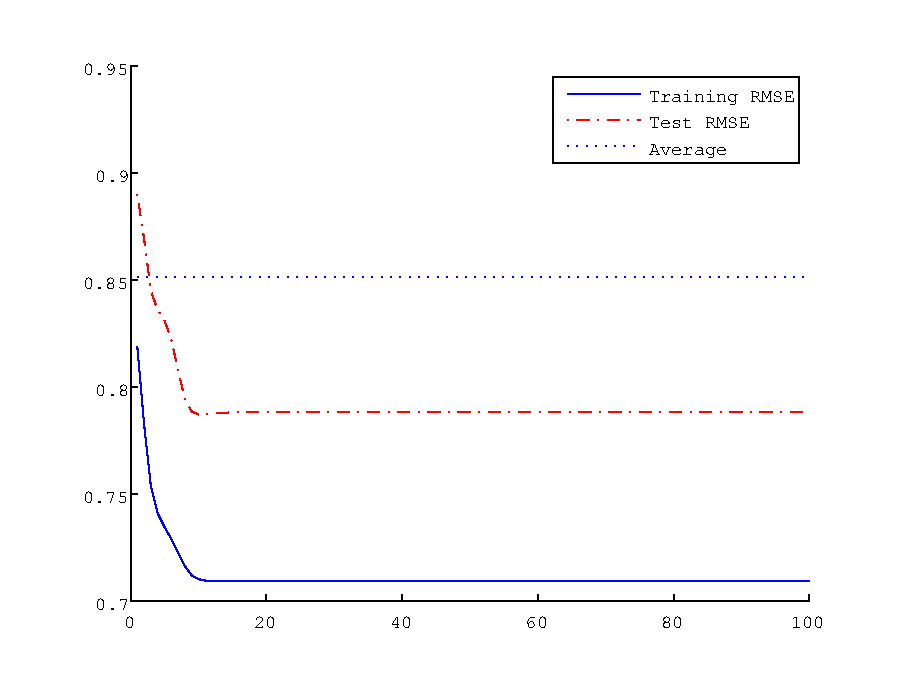
\includegraphics[scale=0.7]{figure/lrem_typical_plot}
  \end{center}
  \caption{Typical result when $d = 2$ and (Ratio of missing element)=0.5. The dotted line shows the RMSE when the estimation is simply the average rating of each movie (i.e. zero-order estimation)}
  \label{fig:lrem_typical_plot}
\end{figure}

Table \ref{table:lrem_result} compares the average RMSE of ten runs with the different dimensions of the low-rank approximation $d$ and the different ratio of the missing element in the rating matrix. Looking at the table in column-wise, it is found that the algorithm works better for the raining data with less missing ratings, which is an obvious result. An interesting result can be found by looking at the table in row-wise; larger dimension results in the larger RMSE when the rating matrix is sparse, but it results in the smaller RMSE when the rating matrix is mostly filled. It is because the algorithm badly overfits to the training data when the number of free parameters are large while the number of the available training data is small. 


\begin{table}[h]
 \caption{RMSE with different dimensions $d$ and different ratio of the missing element. The values are the average of ten runs.}
 \label{table:lrem_result}
 \begin{center}
  \begin{tabular}{|c|c||c|c|c|}
    \hline
    \multicolumn{2}{|c|}{}  & \multicolumn{3}{|c|}{Ratio of missing element in $R$} \\
    \cline{3-5}
     \multicolumn{2}{|c|}{}    &  0.7  &  0.5  & 0.2   \\
    \hline
    \hline
       & 1 &  0.808  &  0.795  &  0.789  \\
    \cline{2-5}
     $d$ & 2 &  0.859  &  0.790  & 0.772   \\
    \cline{2-5}
     & 3 &  0.933  &  0.808  &  0.772  \\
    \hline
  \end{tabular}
 \end{center}
\end{table}

\subsection{Complexity Analysis}
\paragraph{Time complexity} 
The most time consuming part of the algorithm is the $d$ by $d$ matrix inversion $(\check{M}^T\check{M})^{-1}$ in Eq. \ref{eq:lrem_core}. In practice, Gauss Elimination, which has a complexity of $\OO{n^3}$, is used to find the solution instead of complete matrix inversion. The inverse of matrix is computed $n_U+n_M$ times in each iteration. Thus the time complexity of the algorithm is 
\begin{equation}
\OO{d^3N(n_U+n_M)}
\end{equation}
where $N$ is the number of iterations.

\paragraph{Space complexity}
Only U and M are stored during computation. Thus the space complexity is
\begin{equation}
\OO{d(n_U+n_M)}.
\end{equation}

\subsection{Estimated performance on the full Netflix prize data}
\paragraph{Computational cost}
It took about 15 seconds for 100 iteration with $n_U=892$, $n_M=51$, and $d=3$ on Intel Celeron 2.0 GHz CPU. Thus for the full Netflix prize data where $n_U=480,189$ and $n_M=17,770$, the computation time for 100 iterations would take about 2 hours with $d=3$. Requied memory space would be about 11 MByte. Thus this is a tractable algorithm for the full Netflix prize data.

\paragraph{RMSE}
In the actual Netflix prize data 99.9\% elements of the rating matrix are missing. With the small data set where $n_U=892$, $n_M=51$, the algorithm cannot run with 99.9\% sparsity since $(\check{M}^T\check{M})^{-1}$ in Eq. \ref{eq:lrem_core} become singular for most of the rows due to the lack of data. One thing we can tell for sure from Table \ref{table:lrem_result} is that RMSE would be worse than 0.808 for the full Netflix prize data. Trying the algorithm on full data is the future work.



\if c\LaTeXe
\quad
\else
\end{document}
\fi





\section{Comparison}
\label{sec:comparison}
We have implemented two different methods for the collaborative filtering in our final project. 

Mixture model uses discrete multinomial distribution for modeling $\PP{R}{U,M}$, which is a natural way to handle the discrete movie ratings. Its shortcoming is that it regards the ratings as just as "labels", which simply means different classes without any relation each other. However, "ratings" is a linear concept (i.e. in rating domain 5 is closer to 4 than to 1), which cannot be captured by the multinomial distribution. Thus seeing many ratings of 5 does not encourage the rating of 4 any more than the rating of 1.

On the other hand, low-rank approximation works in continuous domain by handling discrete ratings as real numbers. Thus it may make predictions out of the range $\range{5}$, such as $1000$, $2.3$, or $-1$. However, since it is a linear model, it can capture the linear concept of the ratings.  

These differences between two models led to the very different result and performance, although both of them use similar optimization method (EM).


\subsection{RMSE}
RMSE of mixture model is worse than low-rank approximation by large, for all sparsity ratio we have tried. 
- EM performs worse
  - EM always predicts rating 4 because the user-type and movie-type
    priors are all nearly uniform
- EM does not degrade for sparser data

The overall disappointing performance of the EM algorithm was one of
the motivations for looking into an alternative approach, namely
low-rank approximation. It is interesting to note that most of the
leading teams in the competition appear to use a low-rank approximation
approach.

\subsection{Scalability}

We saw that the EM algorithm has slow execution times. In the data set
we used, $n_M = 51$ and $n_U = 892$; on the full data set of nearly
500K users and 17K movies, By our complexity analysis, we project that
running the algorithm on the full Netflix data set would take on the
order of \TODO{}

\section{Conclusion}

\TODO{rewrite to be less of a copy-and-paste from intro?}

We successfully implemented two approaches for collaborative
filtering, an EM algorithm for estimating mixture model parameters,
and a low-rank approximation algorithm.  We analyze these approaches
and evaluate them on a subset of the Netflix Prize data set. We also
included the theoretical basis of each approach and the empirical
results of our experimental evaluation as well as complexity analysis
and discussion of their feasibility for larger-scale problems.

\section{Appendix}

\subsection{Mixture Models}
\label{sec:appendix-mixture}

Here are the variables we're using for the mixture models:

\begin{itemize}
\item $\theta$: the entire set of parameters. TODO explain the sharing
  (but not here)
  \begin{itemize}
  \item $\theta^U_i(u)$: the probability distribution over user types
    $u$ for a user $i$ (think
    of this as a table). This is shared by all user-movie ratings for
    user $i$.
  \item $\theta^M_j(m)$: the probability distribution over movie
    types $m$ for a movie $j$. This is shared by all user-movie ratings for movie $j$.
  \item $\theta^R_{u,m}(r)$: the probability distributions over
    ratings $r$ for user type $u$ and movie type $m$. This is shared
    by all user-movie ratings $i,j$.
  \end{itemize}
\item Dimensions and sets
  \begin{itemize}
  \item $n_U$: number of users
  \item $n_M$: number of movies
  \item $k_U$: number of user types
  \item $k_M$: number of movie types
  \item $I$: the set of indexes $i,j$ of the ratings in the training
    set
  \item $I_T$: the set of indexes $i,j$ of the ratings in the test set
  \end{itemize}
\item Indexes. This allows us to omit ranges in sums and quantifiers.
  \begin{itemize}
  \item $i$: generally used to index over users
  \item $j$: generally used to index over movies
  \item $u$: generally used to index over user types
  \item $m$: generally used to index over movie types
  \end{itemize}
\item Random variables
  \begin{itemize}
  \item $U_i$: the user type of user $i$
  \item $M_j$: the movie type of movie $j$
  \item $R_{i,j}$: the rating user $i$ gave for movie $j$
  \end{itemize}
\end{itemize}

%% Bibliography
%\setlength{\bibsep}{2pt}
\footnotesize
\bibliography{refs}
\bibliographystyle{abbrvnat}

\end{document}

%%%%%%%%%%%%%%%%%%%%%%%%%%%%%%%%%%%%%%%%%%%%%%%%%%%%%%%%%%%%%%%%%%%%%%%%

\begin{comment}

\subsection{Mixture Model 1}

TODO insert graphical model

The likelihood of our model is:

\begin{align*}
  L \left( D \mid \theta \right)
  =& \PP{ R_{1,1} = r_{1,1}, \dots, R_{n,m} = r_{n,m} }{ \theta } \\
  =& \prod_{i,j} \PP{ R_{i,j} = r_{i,j} }{ \theta } \\
  =& \prod_{i,j} \sum_{u,m}
  \PP{ R_{i,j} = r_{i,j} }{ U_i = u, M_j = m, \theta_R }
  \PP{ U_i = u }{ \theta_U }
  \PP{ M_j = m }{ \theta_M } \\
  =& \prod_{i,j} \sum_{u,m} \theta_R(r \mid u,m) \theta_U(u) \theta_M(m)
\end{align*}

E-step:

\begin{align*}
  \forall i,j:
  & \PP{ U_i = u, M_j = m }{ R_{i,j} = r_{i,j}, \theta } \\
  =& \frac{
    \PP{ U_i = u, M_j = m, R_{i,j} = r_{i,j} }{ \theta }
  }{
    \PP{ R_{i,j} = r_{i,j} }{ \theta }
  } \\
% P(U,M|R) = P(U,M,R) = P(R|U,M) P(U,M)
  =& \frac{
    \PP{ U_i = u, M_j = m }{ \theta }
    \PP{ R_{i,j} = r_{i,j} }{ U_i = u, M_j = m, \theta }
  }{
    \sum_{u',m'}
    \PP{ U_i = u', M_j = m' }{ \theta }
    \PP{ R_{i,j} = r_{i,j} }{ U_i = u', M_j = m', \theta }
  } & \textrm{Bayes' rule} \\
  =& \frac{
    \PP{ U_i = u }{ \theta_U }
    \PP{ M_i = m }{ \theta_M }
    \PP{ R_{i,j} = r_{i,j} }{ U_i = u, M_j = m, \theta }
  }{
    \sum_{u',m'}
    \PP{ U_i = u' }{ \theta_U }
    \PP{ M_i = m' }{ \theta_M }
    \PP{ R_{i,j} = r_{i,j} }{ U_i = u', M_j = m', \theta }
  } & \textrm{Bayes' rule} \\
  =& \PP{}{}
\end{align*}

M-step:

\begin{align*}
\forall i,j: &
\PP{ R_{i,j} = r }{ U_i = u, M_j = m, \theta_R } \\
\forall i: &
\PP{ U_i = u }{ \theta_U } \\
=& \frac{
  \N{cells with user type $i$}
}{
  \N{cells}
}\\
=& \N{}
\end{align*}

TODO finish/correct above equations

\end{comment}
